\section{Optimizing Object Tracking}
\label{sec:methods/section_b}

Object tracking pipeline consists of YOLOv3 and SORT, and using the softwares from \cite{jocher_ultralyticsyolov3_2021} and \cite{abewley_abewleysort_2021}, there are 6 parameters needed to be set to run the object tracking. In order to run these softwares, we have to set the suitable parameters, hence, I set the appropriate parameters by optimizing the detection performance for YOLOv3 and tracking performance for SORT. The following parameters needed to be set for YOLOv3 are as follows.
\begin{itemize}
    \item \textbf{Image size}: This parameter is the image resolution for inference of object detection in the YOLOv3 model.
    \item \textbf{Confidence threshold}: This parameter indicates the threshold of object detection. The higher the threshold, the object detector will less likely to detect the target but also less mistakes in detection.
    \item \textbf{IOU threshold for Non-maximum suppression (NMS)}: NMS prevents multiple detections on the same target \cite{redmon_you_2016}. IOU threshold is used in applying NMS in our YOLOv3.
\end{itemize}
For the image size parameter, any input image will be resized to this resolution for prediction. Since the resolution of 640x640 was used in training the pre-trained network weight, we speculated that the detection performance will be the most optimized in that resolution during the inference in testing samples; therefore, we chose 640x640 as an image size.

For the confidence threshold and IOU threshold for NMS, I apply the grid search method to determine the suitable values. To tune these parameters, I run YOLOv3 and SORT on the selected training sequence of Class C PartyScene. Since both parameters range from 0 to 1, I run the detector with a step size of 0.05, and plot the detection performance $F1$ over different confidence threshold and IOU threshold as shown in Figure \ref{fig:optimizing_detector}.
%https://tex.stackexchange.com/questions/278574/common-caption-below-vertically-centered-figure-and-table

\begin{figure}[!tb]
\centering

\begin{tabular}{@{}c@{}}
\resizebox{0.5\linewidth}{!}{
  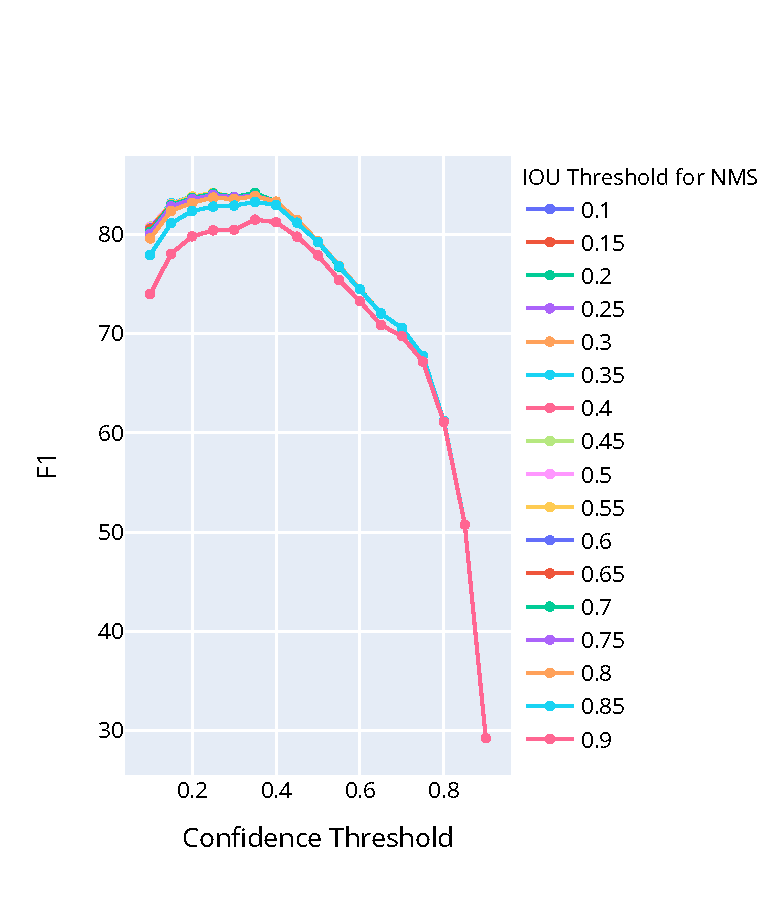
\includegraphics{img/optimizing_detector.pdf}}
\end{tabular}\qquad
\resizebox{0.4\linewidth}{!}{
\begin{tabular}{rrr}
\toprule
 Confidence Threshold &  IOU threshold for NMS &    F1 \\
\midrule
                 0.25 &                   0.35 & 84.20 \\
                 0.25 &                   0.40 & 84.20 \\
                 0.25 &                   0.45 & 84.20 \\
                 0.25 &                   0.50 & 84.20 \\
                 0.25 &                   0.55 & 84.20 \\
\bottomrule
\end{tabular}
}

\caption[Optimizing YOLOv3 by maximizing F1 score on "all" object classes]
{Optimizing YOLOv3 by maximizing F1 score on "all" object classes.}
\label{fig:optimizing_detector}
\end{figure}
The table and plot in this figure shows that there are optimal F1 score over different confidence and IOU threshold. The table in (a) shows that the detector achieved the same F1 score over different IOU threshold at confidence threshold of 0.25. Since the higher the IOU threshold we choose, it makes the detector more careful in detection, or in other words, we expect to see less FP and more FN. Therefore, we chose the confidence threshold of 0.25 and IOU threshold for NMS to be 0.55. Note that I also attempted on tuning the parameters based on optimizing mAP but this metric didn't give me insight in finding optimal values of parameters, as explained in Appendix.

For optimizing the tracking performance of SORT, the following input parameters is listed \cite{bewley_simple_2016}.
\begin{itemize}
    \item \textbf{Max age}: As T\textsubscript{lost} explained in Chapter \ref{sec:background/section_b}, the value of maximum age determines the maximum number of frames to be alive while no objects are detected before the trajectory termination.
    \item \textbf{Min hits}: Minimum number of necessary detections before the trajectory creation and its assignment initialization.
    \item \textbf{IOU threshold}: Minimum IOU threshold for object matching. IOU less than this threshold indicates that the object doesn't overlap enough with the ground truth, so identity will not be assigned, but assignment takes place when IOU is higher than the threshold.
\end{itemize}
For the max age, I chose the value of 1 because \citeauthor{bewley_simple_2016} justified this value by the two reasons; the constant linear motion in Kalman filter framework does not cover the true dynamics where non-linear motion exists and SORT does not deal with the object re-identification \cite{bewley_simple_2016}. 

For the min hits and IOU threshold, I run SORT on the training sequence of Class C PartyScene for both parameters from 0.1 to 0.9 at a step size of 0.05 as a grid search method. To optimize these parameters, I have tested on both cases of tracking; single class of Person only tracking and multiple classes tracking for more general case which includes more discontinuity of detections. I have chosen Person for the tracking in this tuning since I considered Person class is "cleaner" than other classes because the objects are mostly present in the frames without discontinuity of detections, where objects are absent. For the multiple classes tracking case, SORT will track all the classes in the frames, which are available in ground truth. Figure \ref{fig:optimizing_tracker_0} shows the result of Person class tracking and the evaluation based on MOTA over different min hits and IOU threshold is plotted and the highest scores are shown in the table. Although there is no single metric that has been agreed to evaluate the tracking performance, since MOTA is the most popular metric in MOT and it serves as a good indicator for the general tracking performance \cite{bernardin_evaluating_2008} \cite{milan_mot16_2016}, I started from optimizing based on MOTA instead of solving multiple objective optimization problem for all the tracking metrics and t. This result indicates that for the Person tracking, MOTA score is optimal at min hits of 2 and IOU threshold from 0.10 to 0.40. Figure \ref{fig:optimizing_tracker_all} shows that min hits of 9 and IOU threshold from 0.10 to 0.40 achieve the optimal performance.
\begin{figure}[htbp]
  \centering
 
  \begin{subfigure}{1.0\textwidth}
\centering

    \begin{tabular}{@{}c@{}}
    \resizebox{0.5\linewidth}{!}{
      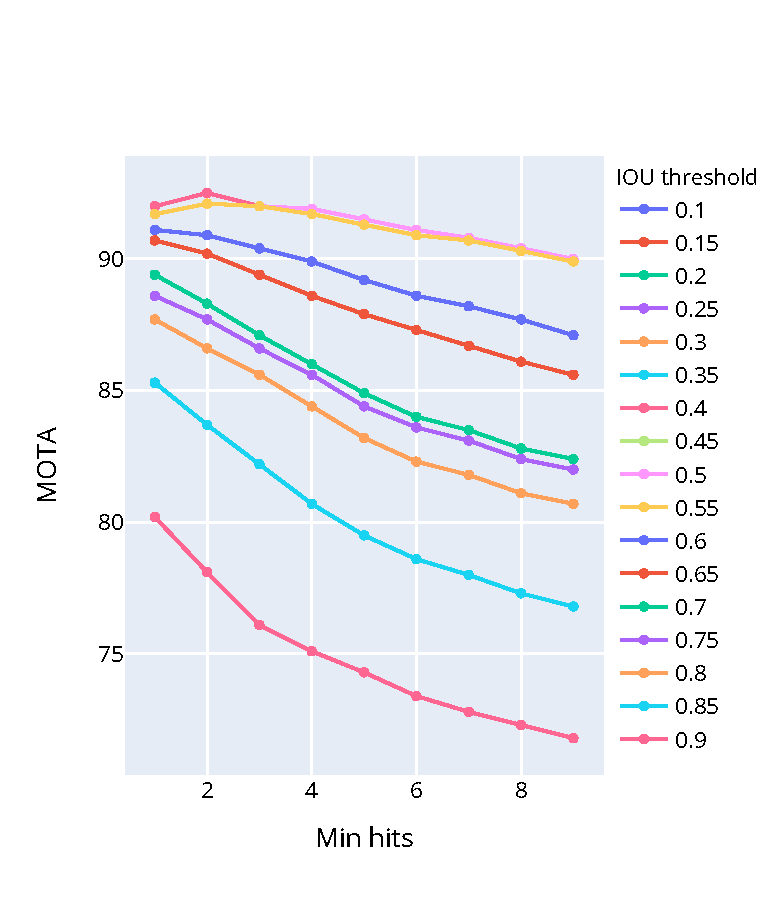
\includegraphics{img/optimizing_tracker_0.pdf}}
    \end{tabular}\qquad
    \resizebox{0.4\linewidth}{!}{
    \begin{tabular}{rrrr}
    \toprule
     Max age &  Min hits & IOU threshold &  MOTA \\
    \midrule
           1 &         2 &       0.10 & 92.50 \\
           1 &         2 &       0.15 & 92.50 \\
           1 &         2 &       0.20 & 92.50 \\
           1 &         2 &       0.25 & 92.50 \\
           1 &         2 &       0.30 & 92.50 \\
           1 &         2 &       0.35 & 92.50 \\
           1 &         2 &       0.40 & 92.50 \\
    \bottomrule
    \end{tabular}
    }
    
    \caption{A caption for a figure in a figure and a table side by side}\label{fig:optimizing_tracker_0}
  \end{subfigure}
 
    \bigskip
 
  \begin{subfigure}{1.0\linewidth}
    \centering
    
    \begin{tabular}{@{}c@{}}
    \resizebox{0.5\linewidth}{!}{
      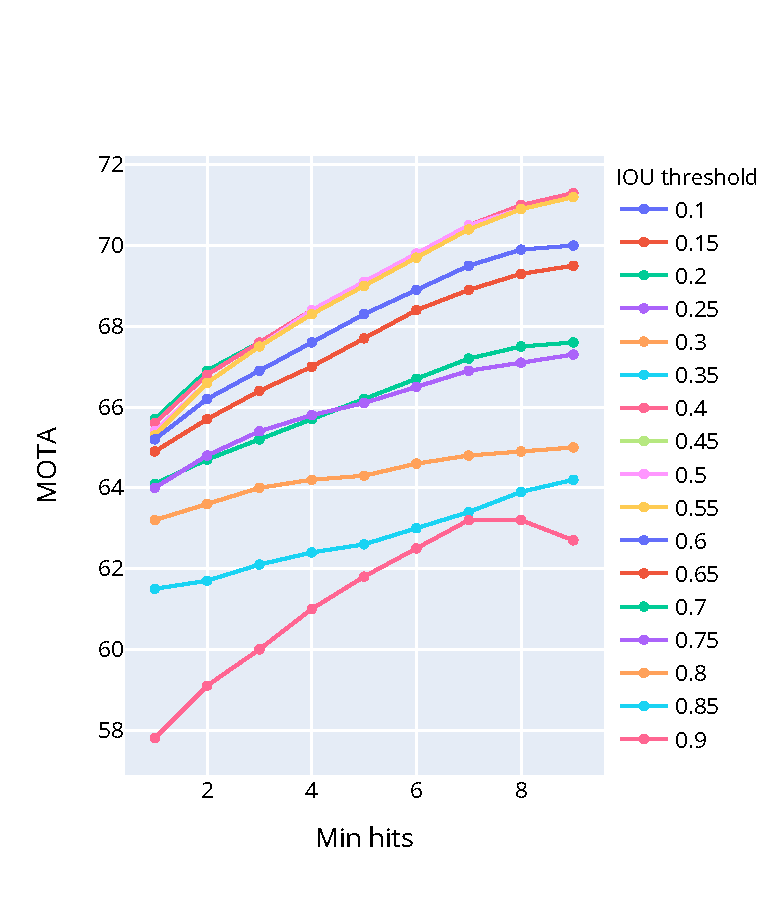
\includegraphics{img/optimizing_tracker_all.pdf}}
    \end{tabular}\qquad
    \resizebox{0.4\linewidth}{!}{
    \begin{tabular}{rrrr}
    \toprule
     Max age &  Min hits &  IOU threshold &  MOTA \\
    \midrule
           1 &         9 &       0.10 & 71.30 \\
           1 &         9 &       0.15 & 71.30 \\
           1 &         9 &       0.20 & 71.30 \\
           1 &         9 &       0.25 & 71.30 \\
           1 &         9 &       0.30 & 71.30 \\
           1 &         9 &       0.35 & 71.30 \\
           1 &         9 &       0.40 & 71.30 \\
    \bottomrule
    \end{tabular}
    }
    
    \caption{A caption for a figure in a figure and a table side by side}\label{fig:optimizing_tracker_all}
  \end{subfigure}
  

  \caption{}
  \label{fig:optimizing_tracker} % label should be placed below caption
\end{figure}
For the IOU threshold selection, I chose 0.4 since both cases of tracking give the best MOTA score at IOU threshold up to 0.4 and the higher the IOU threshold gives the more careful in tracking design. For the min hits, I chose the value of 5 which is the middle between 2 and 9. 

As we have selected the values of parameters based on MOTA; max age of 1, min hits of 5, and IOU threshold of 0.4, the further justification for other metrics is shown in the Appendix A. The selected values of parameters in YOLOv3 and SORT is summarized in Table \ref{tab:parameters}.
\begin{table}[!htbp]
    \centering
    \resizebox{0.4\linewidth}{!}{
    \begin{tabular}{r|r}
    \hline
    YOLOv3 Parameter &  Selected value \\
    \hline
         Image size &               640x640 \\
         Confidence threshold &     0.25 \\
         IOU threshold for NMS &    0.55 \\
    \hline
         SORT Parameter &           Selected value \\
    \hline
         Max age &                  1 \\
         Min hits &                 5 \\
         IOU threshold for matching & 0.4 \\
    \hline
    \end{tabular}
    }
    \caption{Caption}
    \label{tab:parameters}
\end{table}